\documentclass[a4paper,twoside,zihao=5,UTF8]{ctexart}

\ctexset{
	section = {
		format+ = \zihao{-4} \heiti \raggedright,
		name = {,、},
		number = \chinese{section},
		beforeskip = 1.0ex plus 0.2ex minus .2ex,
		afterskip = 1.0ex plus 0.2ex minus .2ex,
		aftername = \hspace{0pt}
	},
	subsection = {
		format+ = \zihao{5} \heiti \raggedright,
		name = {\thesubsection、},
		name = {,、},
		number = \arabic{subsection},
		beforeskip = 1.0ex plus 0.2ex minus .2ex,
		afterskip = 1.0ex plus 0.2ex minus .2ex,
		aftername = \hspace{0pt}
	}
}

\usepackage{blindtext}  
\usepackage{geometry}

% Page margin layout
\geometry{left=2.3cm,right=2cm,top=2.5cm,bottom=2.0cm}


\usepackage{listings}
\usepackage{xcolor}
\usepackage{geometry}
\usepackage{amsmath}
\usepackage{float}
\usepackage{hyperref}

\usepackage{graphics}
\usepackage{graphicx}
\usepackage{subfigure}
\usepackage{epsfig}
\usepackage{float}

\usepackage{algorithm}
\usepackage[noend]{algpseudocode}

\usepackage{booktabs}
\usepackage{threeparttable}
\usepackage{longtable}
\usepackage{listings}
\usepackage{tikz}
\usepackage{multicol}

% cite package, to clean up citations in the main text. Do not remove.
\usepackage{cite}

\usepackage{color,xcolor}

%% The amssymb package provides various useful mathematical symbols
\usepackage{amssymb}
%% The amsthm package provides extended theorem environments
\usepackage{amsthm}
\usepackage{amsfonts}
\usepackage{enumerate}
\usepackage{enumitem}
\usepackage{listings}

\usepackage{indentfirst}
\setlength{\parindent}{2em} % Make two letter space in the first paragraph
\usepackage{setspace}
\linespread{1.5} % Line spacing setting
\usepackage{siunitx}
\setlength{\parskip}{0.5em} % Paragraph spacing setting

% \usepackage[contents =22920202204622, scale = 10, color = black, angle = 50, opacity = .10]{background}

\renewcommand{\figurename}{图}
\renewcommand{\lstlistingname}{代码} 
\renewcommand{\tablename}{表格}
\renewcommand{\contentsname}{目录}
\floatname{algorithm}{算法}

\graphicspath{ {images/} }

%%%%%%%%%%%%%
\newcommand{\StudentNumber}{22920202204622}  % Fill your student number here
\newcommand{\StudentName}{熊恪峥}  % Replace your name here
\newcommand{\PaperTitle}{电子工艺实训}  % Change your paper title here
\newcommand{\PaperType}{实验报告} % Replace the type of your report here
\newcommand{\Date}{2022年6月27日至2022年7月8日}
\newcommand{\Grade}{2020级}
\newcommand{\Department}{计算机科学系}
%%%%%%%%%%%%%

%% Page header and footer setting
\usepackage{fancyhdr}
\usepackage{lastpage}
\pagestyle{fancy}
\fancyhf{}
% This requires the document to be twoside
\fancyhead[LO]{\texttt{\StudentName }}
\fancyhead[LE]{\texttt{\StudentNumber}}
\fancyhead[C]{\texttt{\PaperTitle }}
\fancyhead[R]{\texttt{第{\thepage}页,共\pageref*{LastPage}页}}


\title{\PaperTitle}
\author{\StudentName}
\date{\Date}

\lstset{
	basicstyle          =   \sffamily,          % 基本代码风格
	keywordstyle        =   \bfseries,          % 关键字风格
	commentstyle        =   \rmfamily\itshape,  % 注释的风格,斜体
	stringstyle         =   \ttfamily,  % 字符串风格
	flexiblecolumns,                % 别问为什么,加上这个
	numbers             =   left,   % 行号的位置在左边
	showspaces          =   false,  % 是否显示空格,显示了有点乱,所以不现实了
	numberstyle         =   \zihao{-5}\ttfamily,    % 行号的样式,小五号,tt等宽字体
	showstringspaces    =   false,
	captionpos          =   t,      % 这段代码的名字所呈现的位置,t指的是top上面
	frame               =   lrtb,   % 显示边框
}

\lstdefinestyle{PythonStyle}{
	language        =   Python, % 语言选Python
	basicstyle      =   \zihao{-5}\ttfamily,
	numberstyle     =   \zihao{-5}\ttfamily,
	keywordstyle    =   \color{blue},
	keywordstyle    =   [2] \color{teal},
	stringstyle     =   \color{magenta},
	commentstyle    =   \color{red}\ttfamily,
	breaklines      =   true,   % 自动换行,建议不要写太长的行
	columns         =   fixed,  % 如果不加这一句,字间距就不固定,很丑,必须加
	basewidth       =   0.5em,
}

\lstdefinestyle{CppStyle}{
	language        =   c++,
	basicstyle      =   \zihao{-5}\ttfamily,
	numberstyle     =   \zihao{-5}\ttfamily,
	keywordstyle    =   \color{blue},
	keywordstyle    =   [2] \color{teal},
	stringstyle     =   \color{magenta},
	commentstyle    =   \color{red}\ttfamily,
	breaklines      =   true,   % 自动换行,建议不要写太长的行
	columns         =   fixed,  % 如果不加这一句,字间距就不固定,很丑,必须加
	basewidth       =   0.5em,
}

\algnewcommand\algorithmicinput{\textbf{Input:}}
\algnewcommand\algorithmicoutput{\textbf{Output:}}
\algnewcommand\Input{\item[\algorithmicinput]}%
\algnewcommand\Output{\item[\algorithmicoutput]}%

\usetikzlibrary{positioning, shapes.geometric}

\begin{document}
	
%%%%%%%%%%%%%%%%%%%%%%%%%%%%%%%%%%%%%%%%%%%%
\makeatletter % change default title style
\renewcommand*\maketitle{%
	\begin{center} 
		\bfseries  % title 
		{\LARGE \@title \par}  % LARGE typesetting
		\vskip 1em  %  margin 1em
		{\global\let\author\@empty}  % no author information
		{\global\let\date\@empty}  % no date
		\thispagestyle{empty}   %  empty page style
	\end{center}%
	\setcounter{footnote}{0}%
}
\makeatother
%%%%%%%%%%%%%%%%%%%%%%%%%%%%%%%%%%%%%%%%%%%%
	
	
\thispagestyle{empty}

\vspace*{1cm}

\begin{figure}[h]
	\centering
	
\includegraphics[width=8.0cm]{logo.png}
\end{figure}

\vspace*{1cm}

\begin{center}
	\Huge{\textbf{\PaperType}}
	
	\Large{\PaperTitle}
\end{center}

\vspace*{1cm}

\begin{table}[h]
	\centering	
	\begin{Large}
		\renewcommand{\arraystretch}{1.5}
		\begin{tabular}{p{3cm} p{5cm}<{\centering}}
			姓\qquad 名 & \StudentName  \\
			\hline
			学\qquad号 & \StudentNumber \\
			\hline
			日\qquad期 & \Date  \\
			\hline
			年\qquad级 & \Grade  \\
			\hline
			系\qquad别 & \Department  \\
			\hline
		\end{tabular}
	\end{Large}
\end{table}

\newpage

\title{
	\Large{\textcolor{black}{\PaperTitle}}
}
	
	
\maketitle

\begin{center}
	姓名:\StudentName \qquad 学号:\StudentNumber \qquad 总分:
\end{center}
	
\tableofcontents
 
\newpage
\setcounter{page}{1}

\begin{spacing}{1.2}

\section{PCB制作部分}

\subsection{PCB设计过程及遇到的主要问题}

PCB制作过程和遇到的问题如表~\ref{tbl:pcb}。

\begin{table}[htbp]
	\renewcommand\arraystretch{1.5}
	\centering
	\caption{PCB制作过程和遇到的问题}
	\label{tbl:pcb}
	\begin{tabular}{p{4cm}|p{8cm}}
		\toprule
		\hline
		制作过程 & 问题 \\
		\hline
		原理图绘制 & \begin{minipage}[t]{8cm}
			\begin{enumerate}
				\item 在绘制原理图时连线有虚接的现象。
				\item 没有连接到正确的端口。
			\end{enumerate}
		\end{minipage} 
		
		\\
		\hline
		封装 & \begin{minipage}[t]{8cm}
			\begin{enumerate}
				\item 某些封装没有注意尺寸问题,使得原件安装困难。
				\item 有些封装没有明显标注正负极性,导致安装的时候翻查原理图。
			\end{enumerate}
		\end{minipage} 
		
		\\
		\hline
		布线 & \begin{minipage}[t]{8cm}
			\begin{enumerate}
				\item 没有注意线宽导致线过细,之后进行了修改
				\item 在保证无锐角、无重合的时候遇到了困难,之后重新调整了原件布置顺序
				\item 开关的引脚尺寸不合适
			\end{enumerate}
		\end{minipage} 

		\\
		\hline
		布局 & \begin{minipage}[t]{8cm}
			\begin{enumerate}
				\item 有些部分没有为安装预留足够的空隙
				\item 没有留够助焊区域使得焊接困难
			\end{enumerate}
		\end{minipage} 

		\\
		\hline
		\bottomrule
	\end{tabular}
\end{table}

PCB制作过程中的原理图如图~\ref*{fig:schematic}。

\begin{figure}[H]
	\centering
	\caption{原理图}
	\label{fig:schematic}
	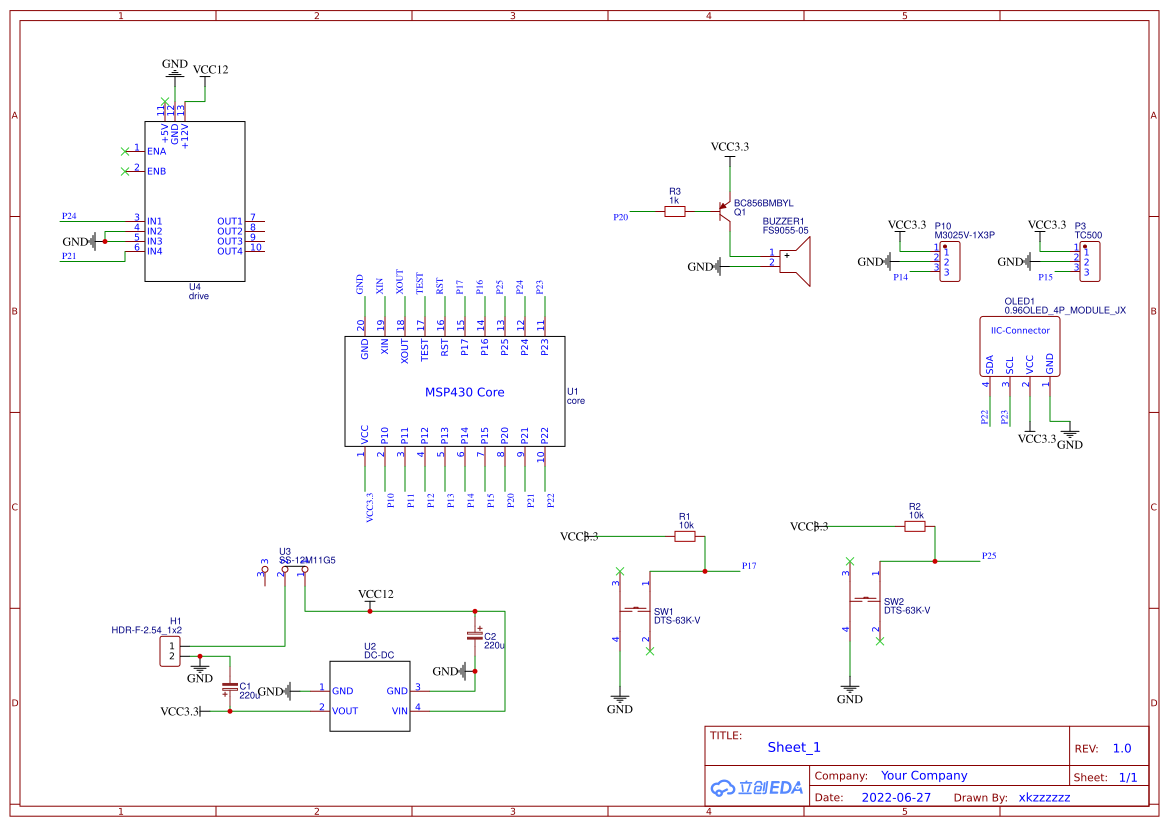
\includegraphics[width=0.5\textwidth]{Schematic.png}
\end{figure}

封装如图~\ref{fig:package},PCB的正反面如图~\ref{fig:pcb}。实物图如图~\ref{fig:real}。

\begin{figure}[htbp]
	\centering
	\caption{封装}
	\label{fig:package}
	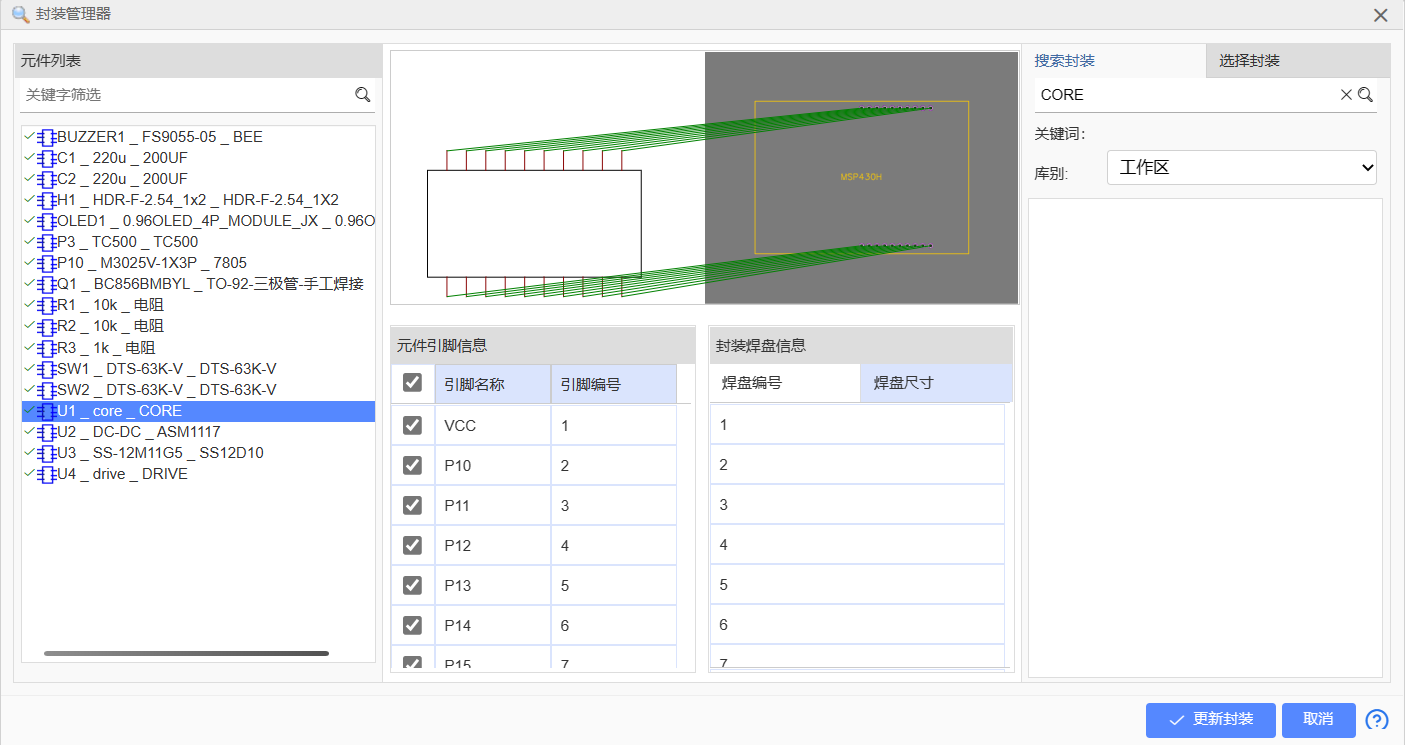
\includegraphics[width=0.6\textwidth]{package.png}
\end{figure}


\begin{figure}[htbp]
    \centering
	\caption{PCB}
	\label{fig:pcb}
	\subfigure[顶部]{
		\begin{minipage}[t]{0.48\linewidth}
			\centering
			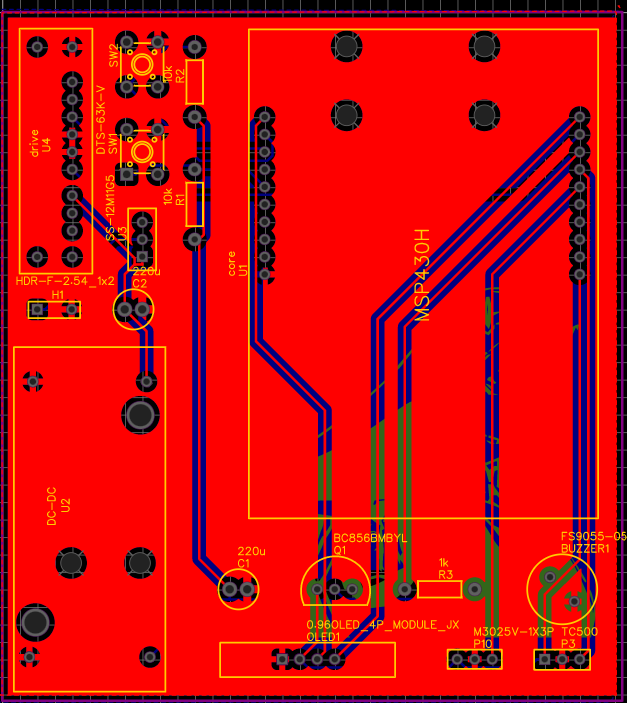
\includegraphics[width=0.8\textwidth]{pcb_top.png}
	\end{minipage}}
	\subfigure[底部]{
		\begin{minipage}[t]{0.48\linewidth}
			\centering
			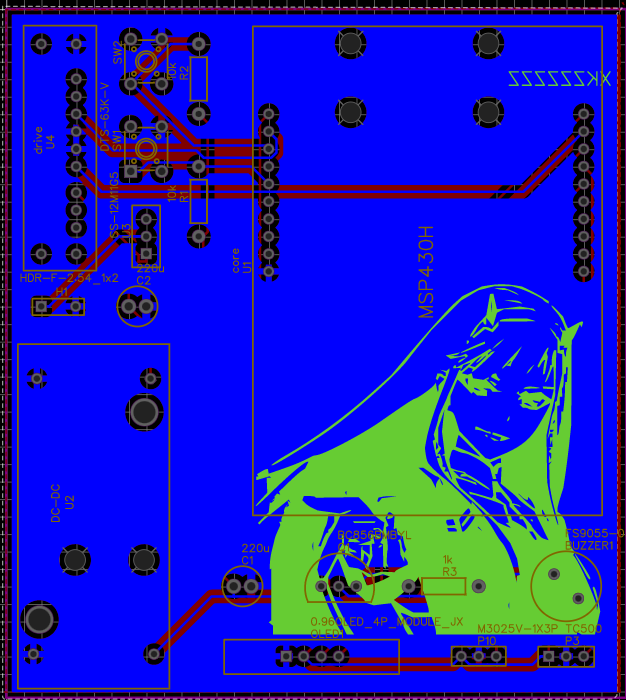
\includegraphics[width=0.8\textwidth]{pcb_bottom.png}
	\end{minipage}}
\end{figure}

\begin{figure}[htbp]
	\centering
	\caption{实物图}
	\label{fig:real}
	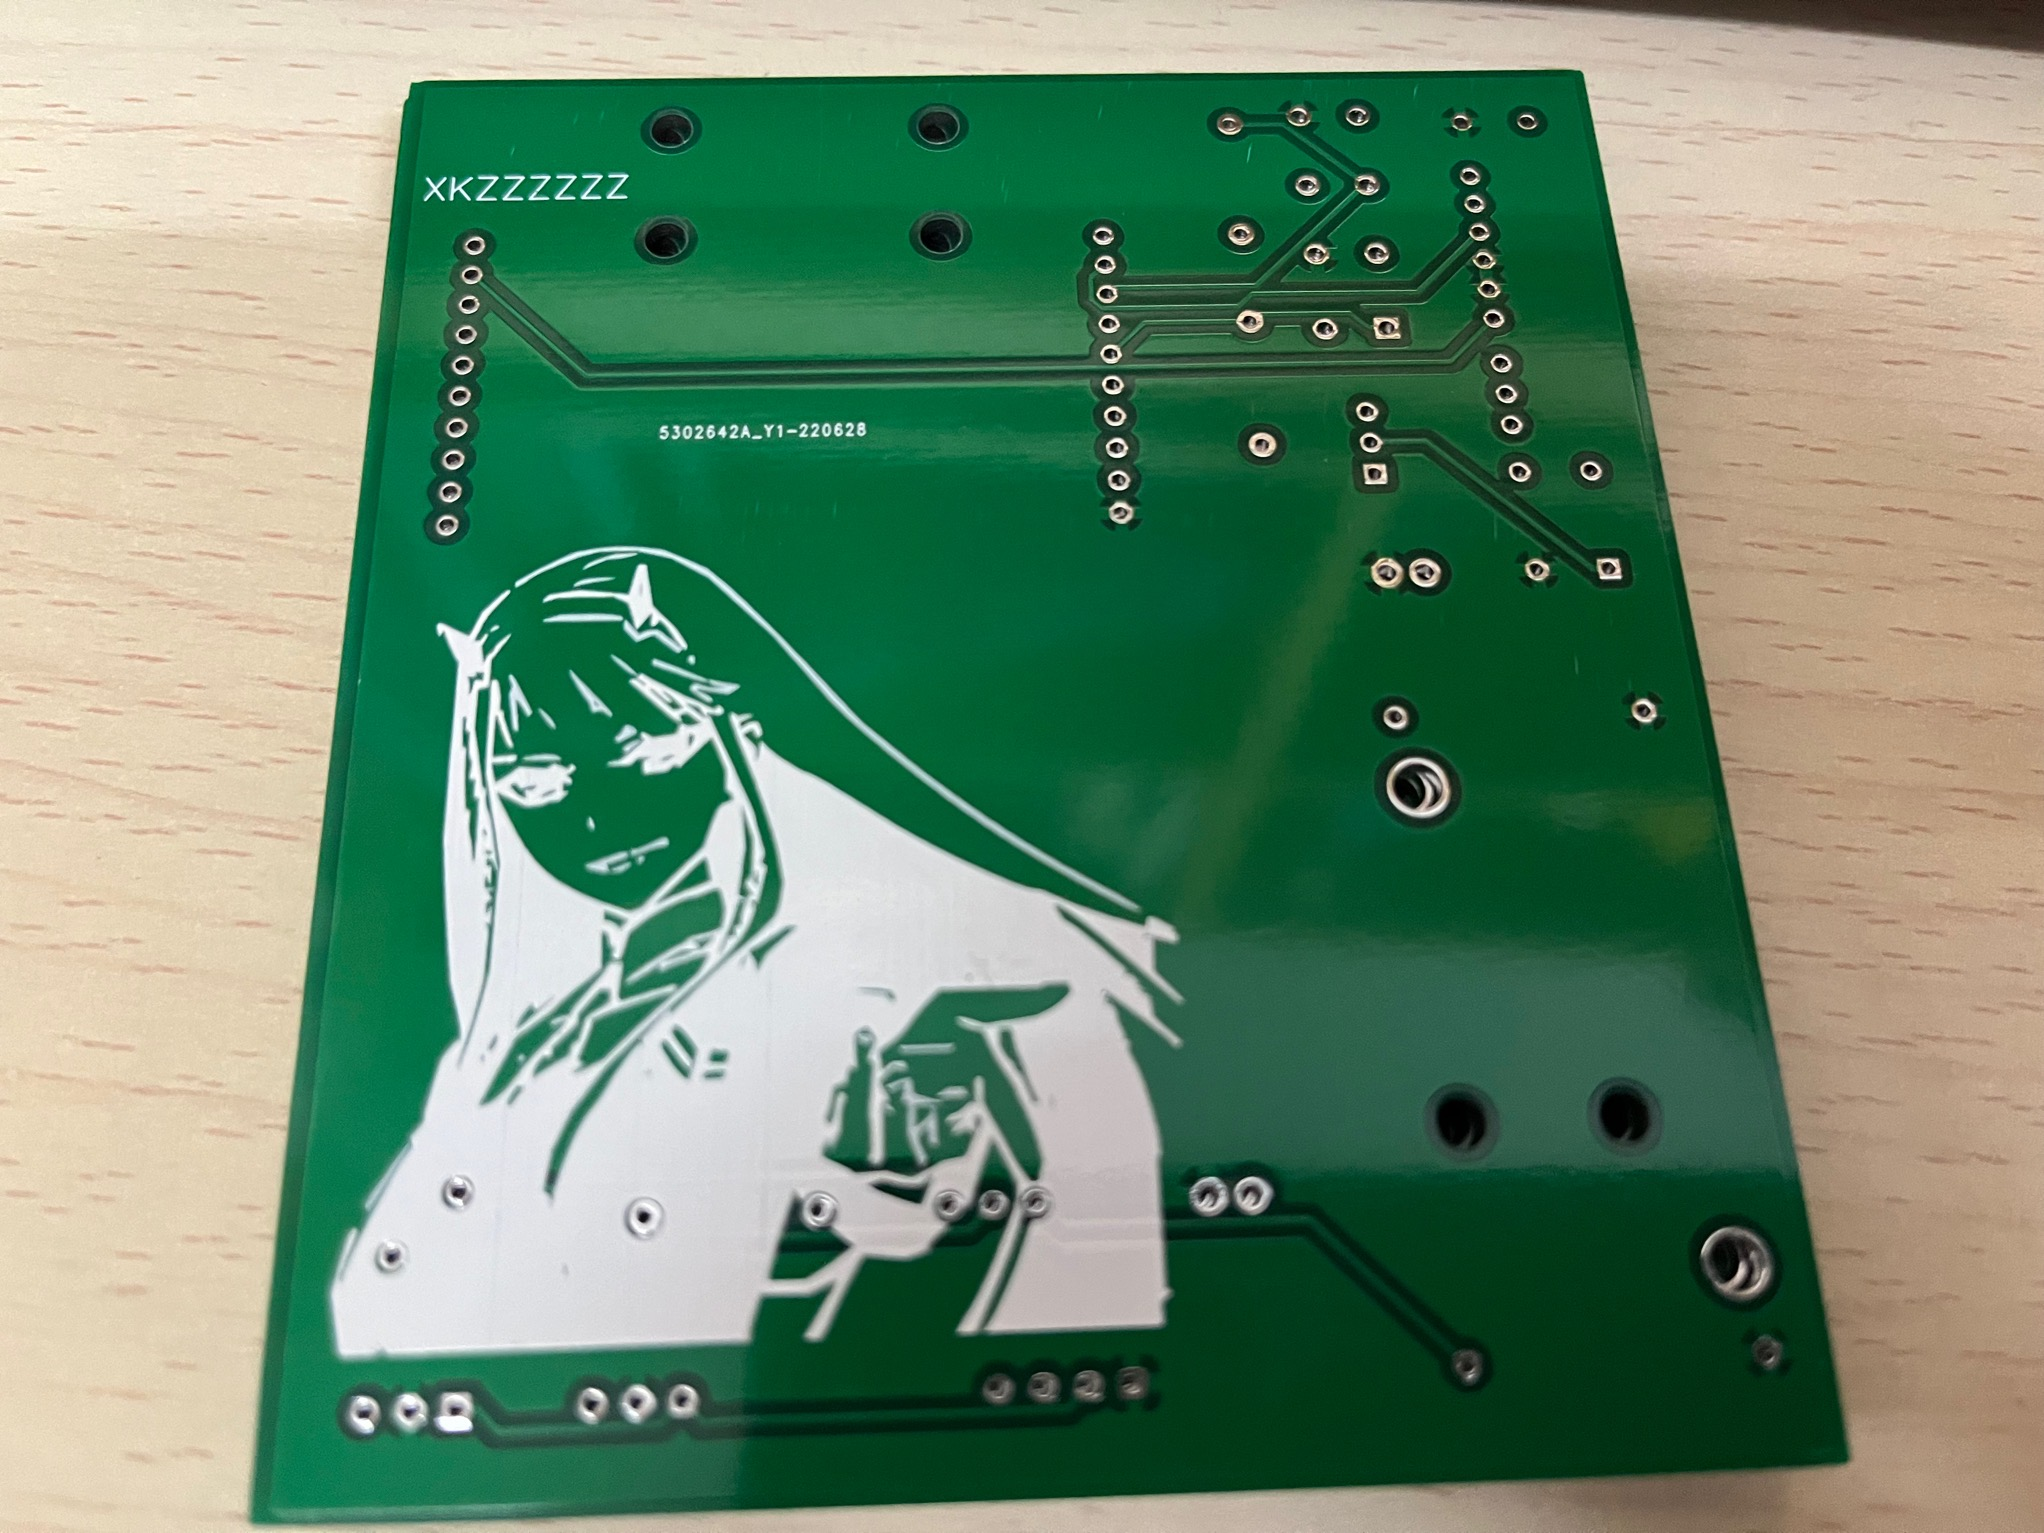
\includegraphics[width=0.6\textwidth]{real.jpg}
\end{figure}


\clearpage
\subsection{注意事项}

\begin{enumerate}
	\item 需要插接导线或者其它线缆的接口元器件一般放到电路板的外侧,
	并且接线的一面要朝外。例如,P1主控板插针一般放到电路板的外侧,
	使单片机接上后多余的部分露在外侧,减少占用PCB板空间。

	\item 元器件就近原则。元器件就近放置,可以缩短PCB导线的距离,
	如果是去耦电容或者滤波电容,越靠近元器件,效果越好。
	例如,H5和SW1就近放置,可以缩短PCB导线距离。

	\item 整齐排列。一个IC芯片的辅助电容电阻电路,围绕此IC把电阻电容整齐的排列,
	可以更美观。例如,R6、R7和C10、C8整齐排列,使整个电路板美观。

	\item 在排列放置元件时,要考虑到实际安装的要求,避免把针脚画反导致需要用线搭接。
\end{enumerate}

\subsection{主要挑战}

\begin{itemize}
	\item 封装:元件封装需要耐心和细心,为了取得良好的效果,我首先在库中寻找符合规格的封装,对封装间隔和引脚对不上的元件,仔细一个个测量修改。
	\item 布局:许多元件需要额外留空间才能放置,如主控板插针需要布局在PCB板外侧,突出的地方可以留在外部减少空间,
	LCD屏幕的位置需要预留出左右两侧较多的空间防止元件与屏幕干涉。
\end{itemize}

\subsection{个人总结和经验感受}

通过两天半的PCB电路板训练,从PCB原理图、封装、原理图库、PCB库、PCB布局、布线、覆铜,通过立创平台提交文件和订单,收到PCB板并运用到小车上,我学习了电路板设计制作和使用的流程。
对PCB的经验总结,就是要仔细地对元器件进行封装和检查,在设计时考虑布局的合理性。立创平台是功能强大的SaaS平台,使用非常方便,既有丰富的元件库,而且操作简单便捷,无需额外安装。
这两天半学到的技能对日后参加比赛、制作电子器件有很大的帮助。

\section{MSP430单片机部分}

\subsection{作业1}
读取 MSP430G2553 LaunchPad 上S2的按键状态,并用该按键控制LED1。按键按下时让LED 1亮起,按键松开时让LED 1熄灭。

\begin{lstlisting}[language=c++,numbers=left,style=CppStyle,caption=作业1,label={code:p1}]
#include <msp430.h> 
int main(void)
{
    WDTCTL = WDTPW | WDTHOLD;    // stop watchdog timer

    P1DIR |= BIT0;
    P1DIR &= ~BIT3;
    P1OUT|=BIT3;
    P1REN |= BIT3;

    while(1)
    {
        if(!(BIT3 & P1IN))
            P1OUT |= BIT0;
        else
            P1OUT &= ~BIT0;
    }
    return 0;
}
\end{lstlisting}

\subsubsection{现象和讨论}
MSP430G2553 LaunchPad 上 S2按键按下时让 LED 1亮起,按键松开时让 LED 1熄灭。
按键S2对应P1.3端口,设置P1.3为输入,LED1对应P1.0端口,设置P1.0为输出,使得按下S2时,
P1.0输出为0,让灯亮,松开时,P1.0输出为1,让灯灭。

在实现上,由于该程序比较简单,没有复杂的需求,对资源管理的要求不高,所以直接轮询而不是使用中断。
但这种方式可能浪费CPU资源,在更复杂的程序中应该使用中断。

\subsection{作业2}
在上一节Blink程序的基础上,将MCLK分别设置为1MHz和8MHz
并观察LED1闪烁的频率有何变化。

\begin{lstlisting}[language=c++,numbers=left,style=CppStyle,caption=作业2,label={code:p2}]

#include <msp430g2553.h>

void set_1mhz()
{
  BCSCTL1 = CALBC1_1MHZ; // Set range

  DCOCTL = CALDCO_1MHZ;

  BCSCTL2 &= ~(DIVS_3); // SMCLK = DCO = 1MHz
}

void set_8mhz()
{
  BCSCTL1 = CALBC1_8MHZ; // Set range

  DCOCTL = CALBC1_8MHZ;

  BCSCTL2 &= ~(DIVS_3); // SMCLK = DCO = 1MHz
}

int main()
{
  WDTCTL = WDTPW | WDTHOLD; // stop watchdog timer
  P1DIR |= 0x01;            // configure P1.0 as output

  set_1mhz();
  //set_8mhz();

  volatile unsigned int i; // volatile to prevent optimization

  while (1)
  {
    P1OUT ^= 0x01; // toggle P1.0
    for (i = 10000; i > 0; i--)
      __delay_cycles(10); // delay
  }
  return 0;
}
\end{lstlisting}

\subsubsection{现象和讨论}
通过对比将主时钟设为1MHz和8MHz的情况下,能明显感觉到8MHz下LED1闪烁频率比1MHz快。
通过改变主时钟频率来改变运行速度从而改变时钟的频率。


\subsection{作业3}
通过GPIO中断的方式,用两个按键分别控制两盏不同的LED灯。每按下一次按键,相应的LED灯改变一次亮灭状态。
提示:板子上只有一个按键S2,可以用杜邦线一端连接在GND或者VCC,另外一端触碰下自己选择的IO口,模拟按键按下的状态。


\begin{lstlisting}[language=c++,numbers=left,style=CppStyle,caption=作业3,label={code:p3}]

#include <msp430.h> 
#if defined(__TI_COMPILER_VERSION__) || defined(__IAR_SYSTEMS_ICC__)
#pragma vector=PORT1_VECTOR
__interrupt void Port_1(void)
#elif defined(__GNUC__)
void __attribute__((interrupt(PORT1_VECTOR))) Port_1(void)
#else
#error Compiler not supported!
#endif
{
    if(!(P1IN & BIT4))
    {
        P1OUT ^= BIT0;
        P1IFG &= ~BIT4;
    }
    if(!(P1IN & BIT5))
    {
        P1OUT ^= BIT6;
        P1IFG &= ~BIT5;
    }

}

int main(void)
{
    WDTCTL = WDTPW + WDTHOLD;   // stop watchdog timer
    P1DIR |= BIT0;
    P1OUT &= ~BIT0;

    P1DIR |= BIT6;
    P1OUT &= ~BIT6;

    P1DIR &= ~BIT4;
    P1OUT != BIT4;
    P1REN |= BIT4;

    P1DIR &= ~BIT5;
    P1OUT != BIT5;
    P1REN |= BIT5;

    P1IES |= BIT4;
    P1IFG &= ~BIT4;
    P1IE |= BIT4;

    P1IES |= BIT5;
    P1IFG &= ~BIT5;
    P1IE |= BIT5;

    __bis_SR_register(GIE);
    return 0;
}
\end{lstlisting}


\subsection{作业4}
编程实现:利用定时器编写呼吸灯。所谓呼吸灯是指LED在一个周期内先逐渐变亮,再逐渐变暗。

\begin{lstlisting}[language=c++,numbers=left,style=CppStyle,caption=作业4,label={code:p4}]

#include <msp430g2553.h>

int IncDec_PWM = 1;

int main(void)
{

  /*** Watchdog timer and clock Set-Up ***/
  WDTCTL = WDTPW + WDTHOLD; // Stop watchdog timer
  DCOCTL = 0;               // Select lowest DCOx and MODx
  BCSCTL1 = CALBC1_1MHZ;    // Set range
  DCOCTL = CALDCO_1MHZ;     // Set DCO step + modulation

  P1DIR |= BIT6;
  P1SEL |= BIT6;

  /*** Timer0_A Set-Up ***/
  TA0CCR0 |= 1000;           // PWM period
  TA0CCR1 |= 1;              // TA0CCR1 PWM duty cycle
  TA0CCTL1 |= OUTMOD_7;      // TA0CCR1 output mode = reset/set
  TA0CTL |= TASSEL_2 + MC_1; // SMCLK, Up Mode (Counts to TA0CCR0)

  /*** Timer1_A Set-Up ***/
  TA1CCR0 |= 2000;           // Counter value
  TA1CCTL0 |= CCIE;          // Enable Timer1_A interrupts
  TA1CTL |= TASSEL_2 + MC_1; // SMCLK, Up Mode (Counts to TA1CCR0)

  _BIS_SR(LPM0_bits + GIE); // Enter Low power mode 0 with interrupts enabled

  return 0;
}

#pragma vector = TIMER1_A0_VECTOR // Timer1 A0 interrupt service routine
__interrupt void Timer1_A0(void)
{

  TA0CCR1 += IncDec_PWM * 2;
  if (TA0CCR1 > 998 || TA0CCR1 < 2)
    IncDec_PWM = -IncDec_PWM;
}
\end{lstlisting}

\subsection{作业5}
编写接收程序和发送程序,当开发板串口接收到PC机发来的字符“1”时,点亮LED1,并向PC机发送“LED\_ON”;
当当开发板串口接收到PC机发来的字符“0”时,熄灭LED1,并向PC机发送“LED\_OFF”;当收到其它字符时,翻转LED1状态,
并向PC机发送“LED\_ON”或者“LED\_OFF”,表明LED1当前的状态。

\begin{lstlisting}[language=c++,numbers=left,style=CppStyle,caption=作业5,label={code:p5}]

#include <msp430g2553.h>
#include <stdint.h>
#include <stdbool.h>

void set_1mhz()
{
  BCSCTL1 = CALBC1_1MHZ; // Set range

  DCOCTL = CALDCO_1MHZ;
}

void uart_init()
{
  UCA0CTL1 |= UCSSEL_2;
  UCA0BR0 = 104;
  UCA0BR1 = 0;
  UCA0MCTL = UCBRS0;
  UCA0CTL1 &= ~UCSWRST;
  IE2 |= UCA0RXIE;
}

void uart_puts(char *c)
{
  while (*c)
  {
    while (!(IFG2 & UCA0TXIFG))
    {
      __nop();
    }
    UCA0TXBUF = *c++;
  }
}

void __attribute__((interrupt(USCIAB0RX_VECTOR))) uart_rx_isr()
{
  volatile int led_on = !!UCA0RXBUF;

  if (led_on)
  {
    P1OUT |= BIT0;
    uart_puts("LED ON\n");
  }
  else
  {
    P1OUT &= ~BIT0;
    uart_puts("LED OFF\n");
  }
}

int main()
{
  WDTCTL = WDTPW | WDTHOLD; // stop watchdog timer

  P1DIR |= BIT0; // configure P1.0 as output
  P1OUT &= ~BIT0;

  DCOCTL = 0;
  set_1mhz();

  P1SEL = BIT1 | BIT2;
  P1SEL2 = BIT1 | BIT2;

  uart_init();

  __bis_SR_register(LPM0_bits | GIE);
  return 0;
}
\end{lstlisting}


\subsection{作业6}

按如下格式在OLED屏上显示自己的姓名、学号和系别信息。

\begin{lstlisting}[language=c++,numbers=left,style=CppStyle,caption=作业6,label={code:p6}]

#include "msp430g2553.h"
#include"I2C_OLED.H"
#include"zimo.h"

#define LEN(arr) (sizeof(arr)/sizeof(arr[0]))

int name_indexes[]={1,2,7,8,9};
int major_indexes[]={5,6,10,11,12,13,14};
int sid[]={2,2,9,2,0,2,0,2,2,0,4,6,2,2};

int main(void)
{
   system_clock();
   I2C_OLED_Init();
   while(1)
   {
	   OLED_All(0);
//	   delay_ms(500);


	   volatile int i=0,cnt=0;
	   for(i=0;i<LEN(name_indexes);i++)
	   {
	       OLED_P16x16Ch((cnt++)*16,0,name_indexes[i]);
	   }

	   i=cnt=0;
	   for(i=0;i<LEN(major_indexes);i++)
	   {
	       OLED_P16x16Ch((cnt++)*16,3,major_indexes[i]);
	   }

	   OLED_P16x16Ch(0,6,3);
	   OLED_P16x16Ch(16,6,4);
	   OLED_P6x8Str(32,6,"22920202204622");

	   for(;;);
   }
}
\end{lstlisting}


\section{基于MSP430的智能小车行驶}

\subsection{电路与程序设计}

\subsubsection{需求分析}

\begin{figure}[htbp]
    \centering
	\caption{小车赛道}
	\label{fig:pcb}
	\subfigure[赛道示意图]{
		\begin{minipage}[t]{0.48\linewidth}
			\centering
			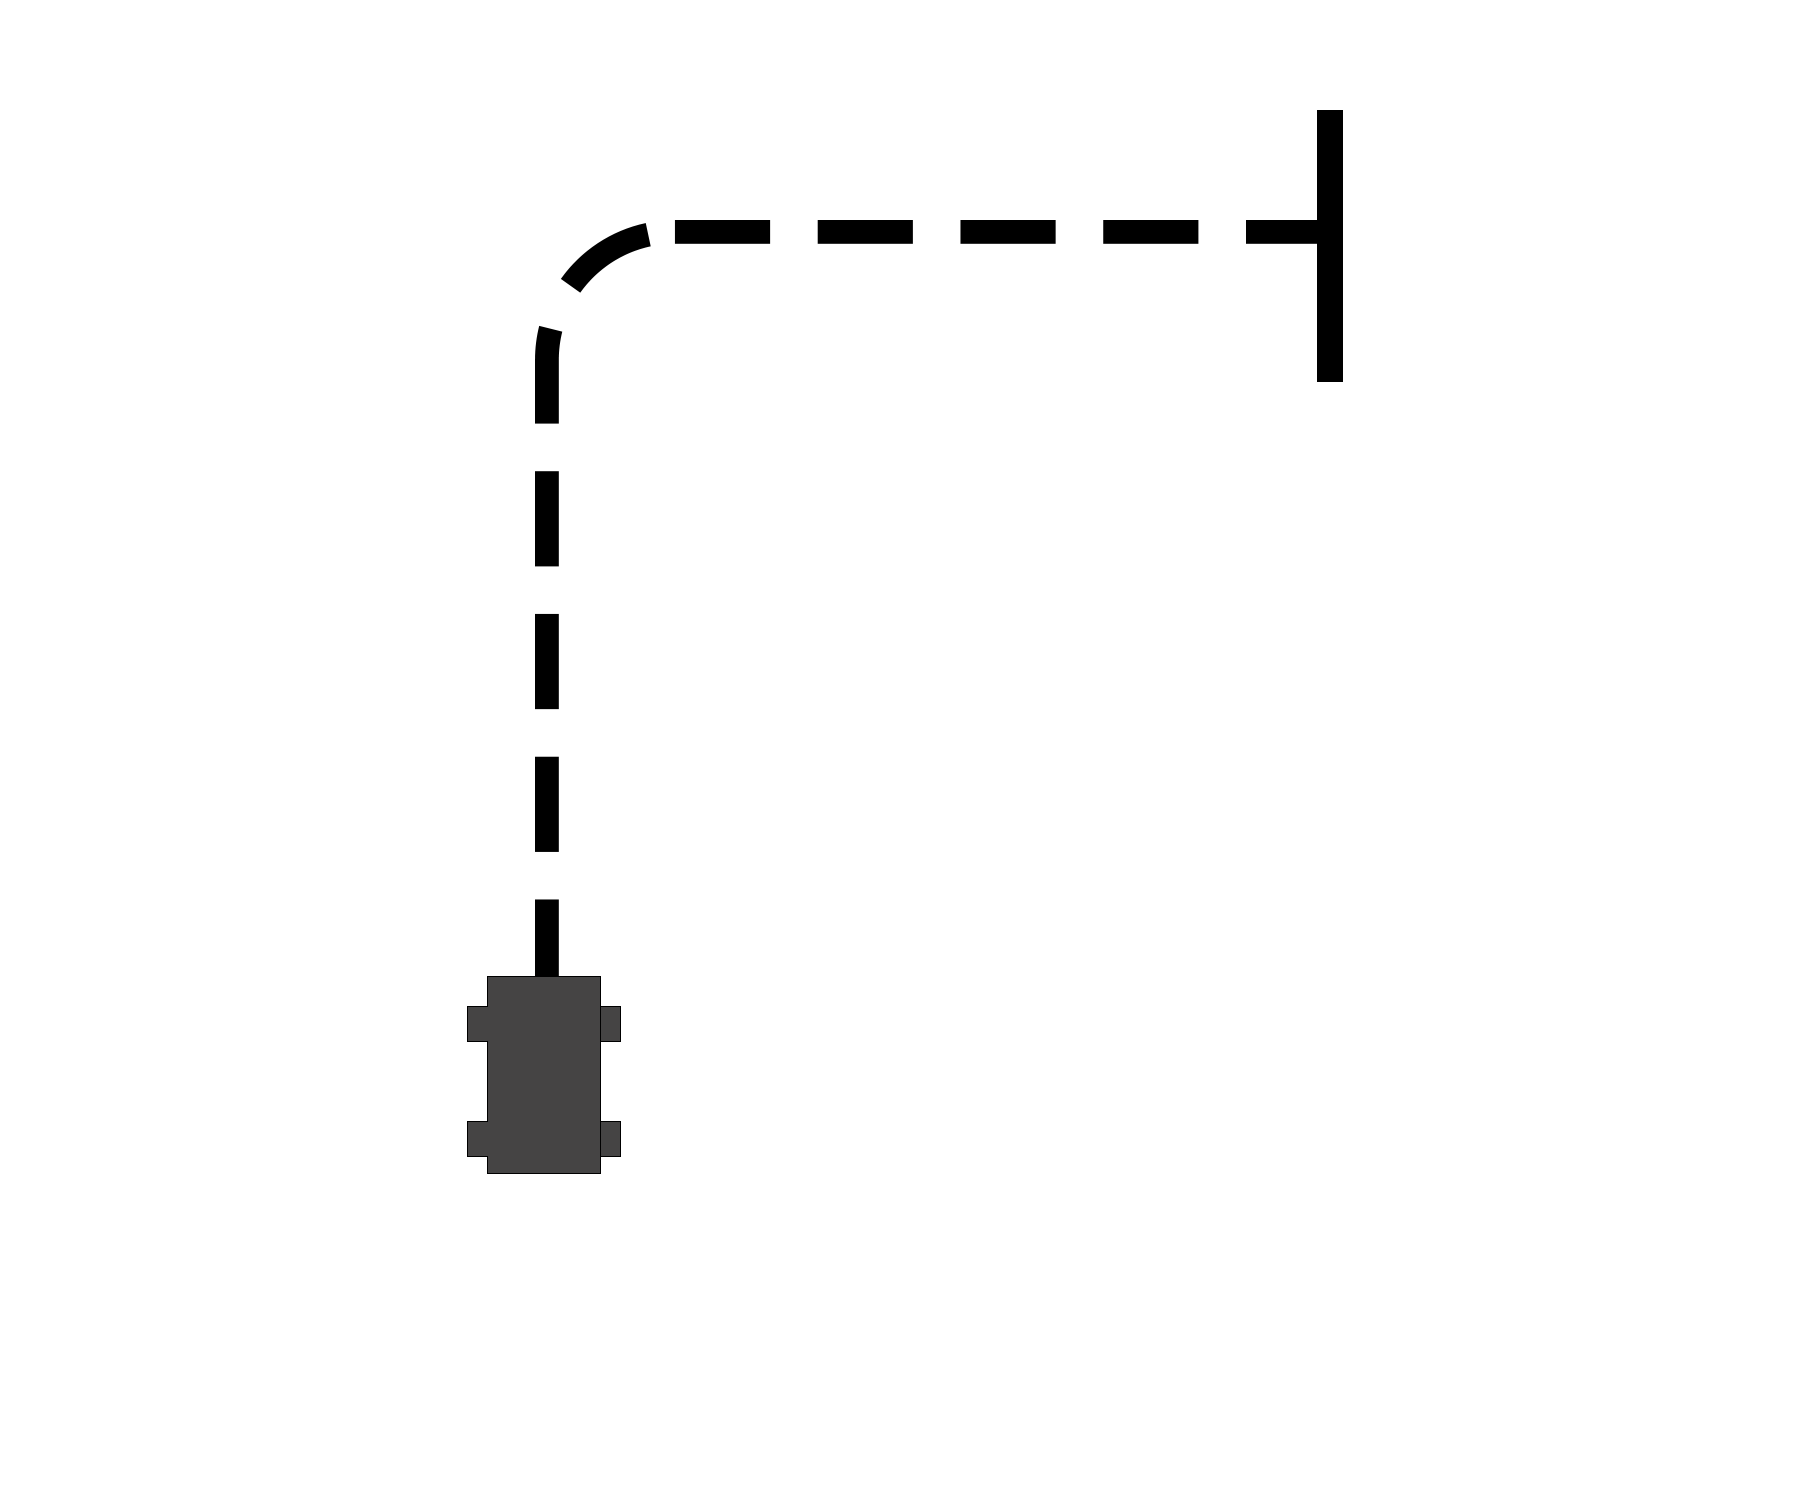
\includegraphics[width=0.8\textwidth]{car_track.png}
	\end{minipage}}
	\subfigure[轨迹示意图]{
		\begin{minipage}[t]{0.48\linewidth}
			\centering
			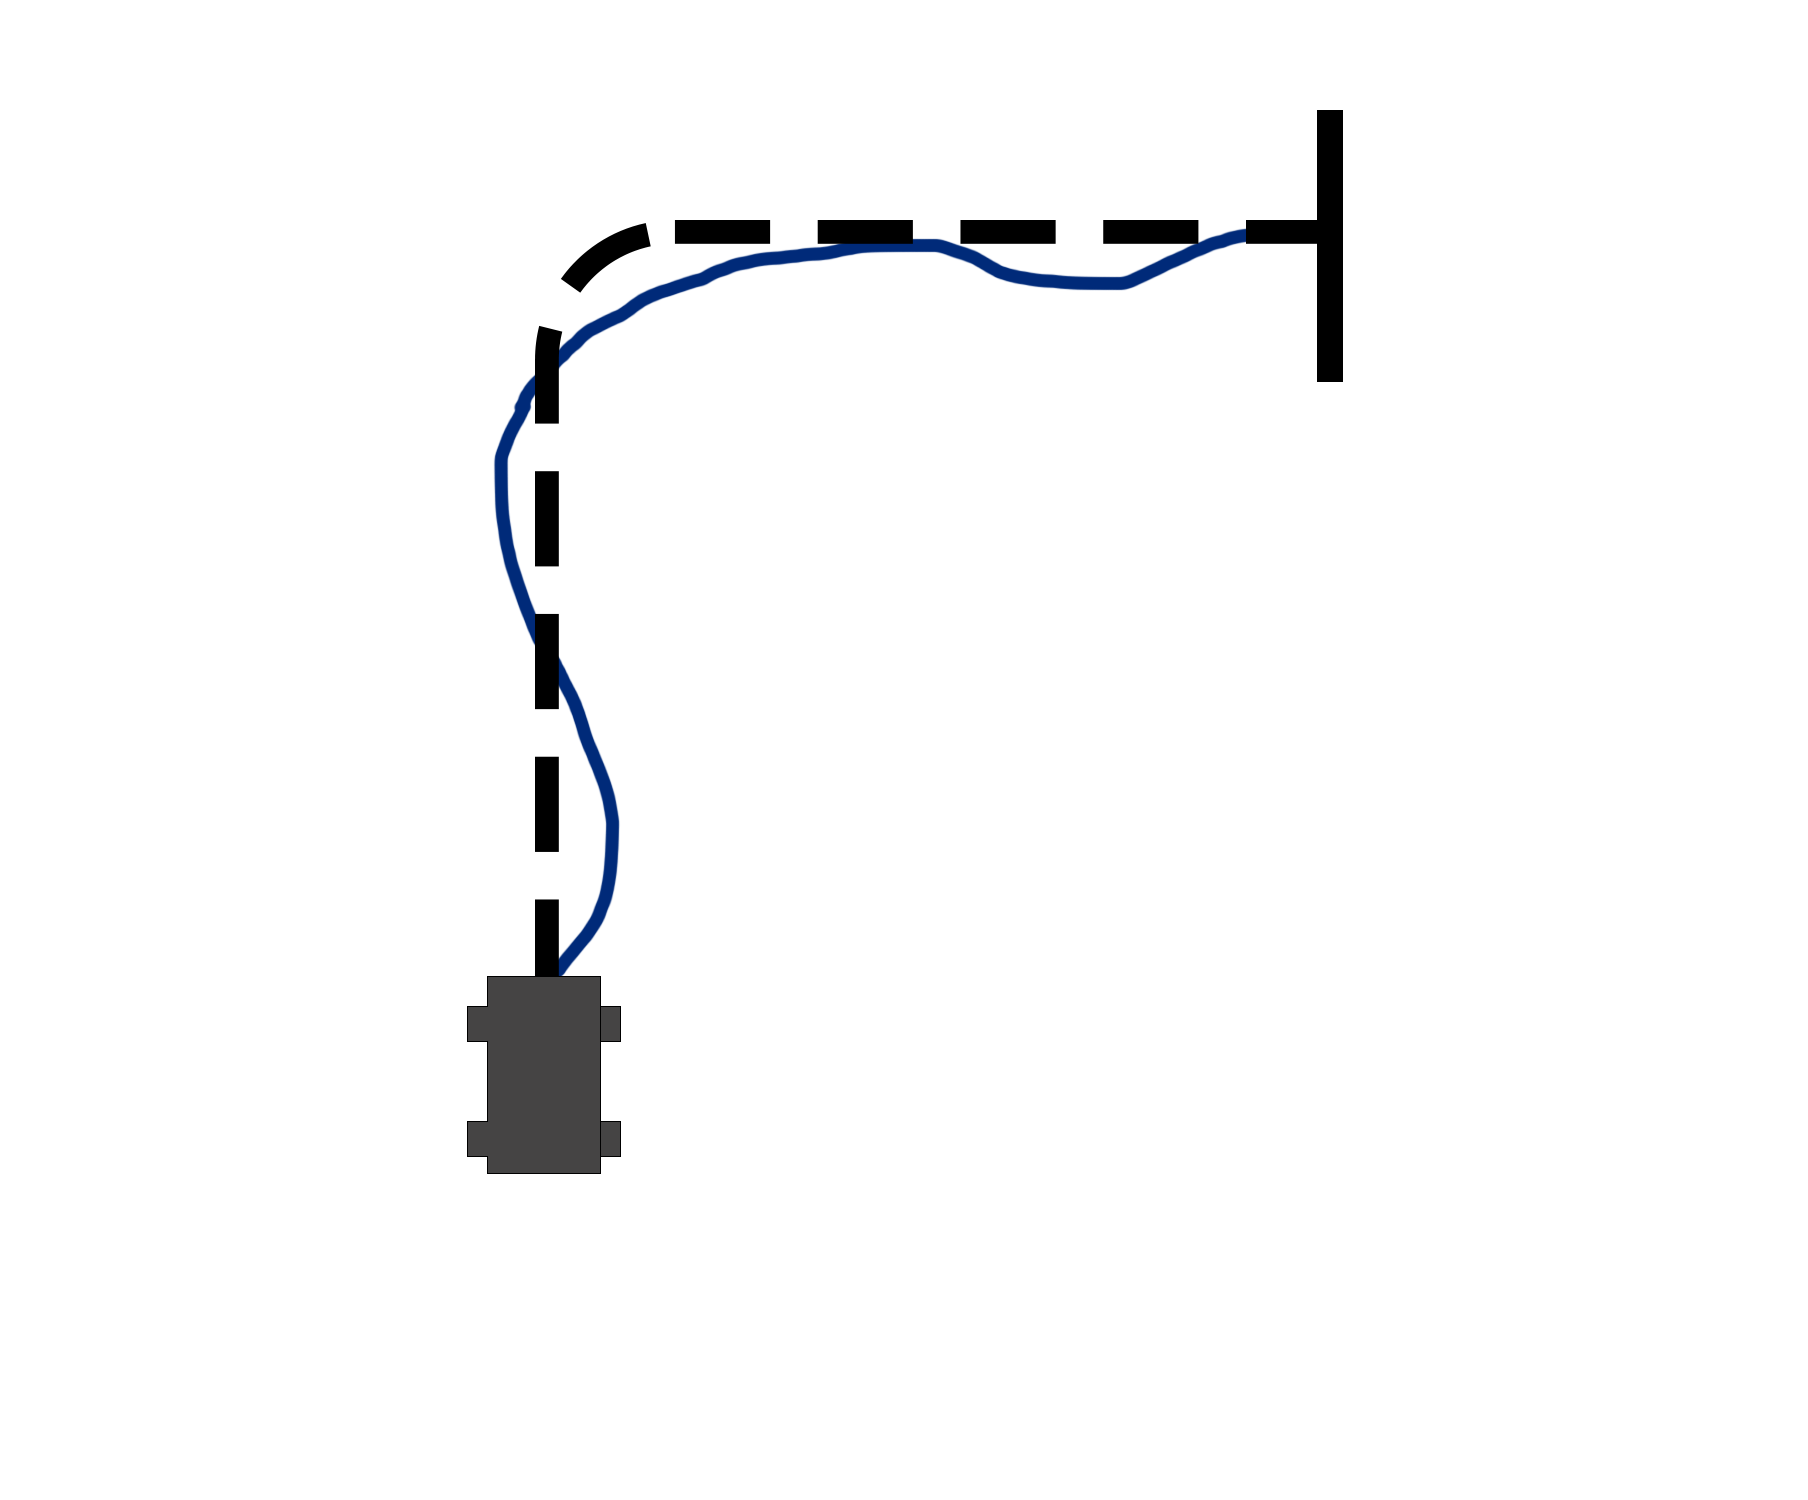
\includegraphics[width=0.8\textwidth]{car_track_example.png}
	\end{minipage}}
\end{figure}

\subsubsection{设计思路}

\subsubsection{非对称的转向参数}

\subsubsection{递增的转向速度加权}

\begin{table}[htb]
	\centering
	\caption{加权函数}
	\label{tbl:weight}
	\renewcommand\arraystretch{1.5}
	\begin{tabular}{c|c}
		\toprule
		\hline
		权函数类型 & 表达式 \\
		\hline
		余弦型函数 & $y(k;n)=\cos(nk\pi)$ \\
		\hline
		多项式型函数 & $y(k;n)=a_nk^n+a_{n-1}k^{n-1}+\cdots+a_1k+a_0$ \\
		\hline
		指数型函数 & $y(k;a,m,n)=m\cdot a^k+n$ \\
		\hline
		\bottomrule
	\end{tabular}
\end{table}

\begin{equation}
	\begin{aligned}
		y(k;a,m,n)=m\cdot a^k+n
	\end{aligned}
\end{equation}

\begin{equation}
	y(k)=a\cdot y(k-1)+b
\end{equation}

\begin{figure}
	\centering
	\caption{函数图像}
	\label{fig:weight}
	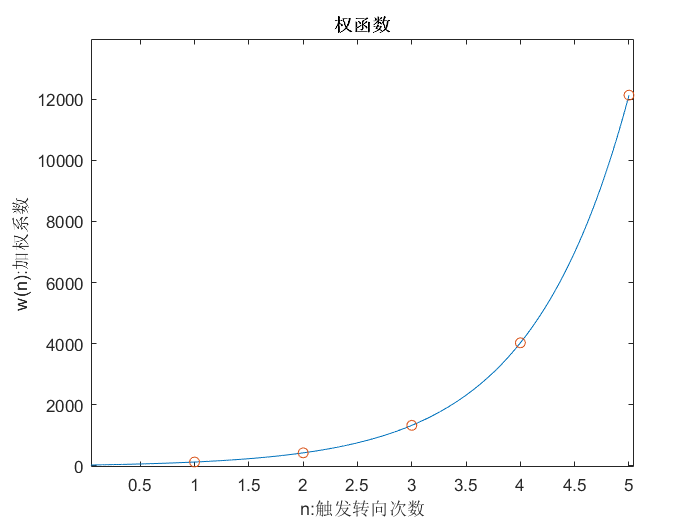
\includegraphics[width=0.8\textwidth]{weight.png}
\end{figure}

\subsubsection{方案总结}

\subsection{测试方案与测试结果}

\subsection{本人所做的工作}

\subsection{经验总结与个人感受}


\section{人工智能入门}


\section{实验改进建议}


\section{实训总结}


\end{spacing}

\end{document}